\chapter{Results}\label{ch:results}

\section{Pre-Pilot Trajectories}\label{sec:prepilot}

Figure~\ref{fig:eventtime} reports event-time contrasts relative to the last pre-pilot year. Each point subtracts the comparison crops' mean log change from the treated crops' mean log change over the same interval. Pre-pilot contrasts near zero would be consistent with parallel observed changes, whereas systematic differences raise concerns about the national comparison. The reference contrast is fixed at zero by construction.

The pre-pilot yield contrasts lie between approximately \textminus 0.04 and 0.03 log points. The joint test has p = 0.88 and does not reject at the 5 percent level. Its power and calibration are limited by the small number of treated crops.

Area and production show more pronounced pre-pilot differences. Their contrasts are approximately \textminus 0.2 log points in earlier years and closer to zero near the reference year, indicating that treated crops gained relative to their comparisons before insurance. The exploratory joint p-values are 0.06 for area and 0.03 for production: only production crosses the stated 5 percent threshold. Both paths remain relevant to assessing comparability, regardless of that threshold. Their similarity is consistent with the accounting relationship between area, yield, and production.

\begin{figure}[htbp]
\centering
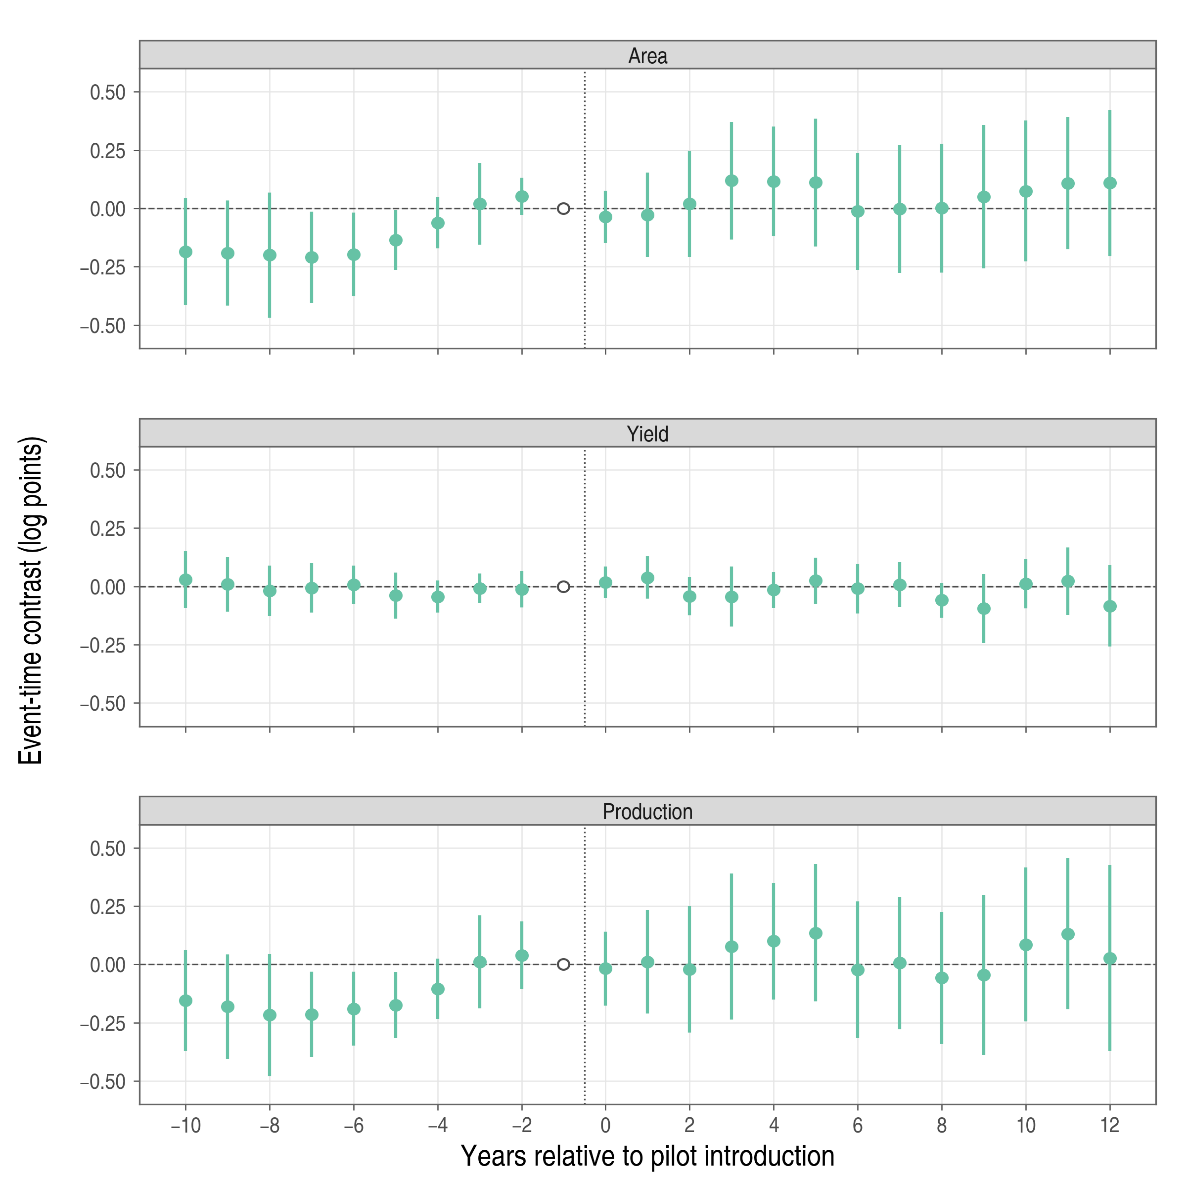
\includegraphics[width=5.40in]{figures/fig6_event_time_contrasts.png}
\caption{Event-Time Contrasts for Cultivated Area, Yield, and Production}\label{fig:eventtime}
\notes{Event-time contrasts relative to the last pre-pilot year (open circle), averaged over the seven treated crops. Bars are 95 percent intervals from 9,999 Webb multiplier draws (Appendix~\ref{app:inference}). The vertical dotted line separates pre-pilot and post-pilot years; post-pilot years include the transition years between the pilot and expansion.}
\end{figure}

Area and production gained relative to comparison crops before the pilots. A reference year close to introduction consequently measures subsequent changes from a later point in that divergence. Section~\ref{sec:sensitivity} examines how alternative reference periods change the reported contrasts.

\section{Aggregate and Crop-Level Contrasts}\label{sec:aggregate}

Table~\ref{tab:main} reports the main contrasts for the full comparison pool and for a pool that excludes spring napa cabbage and spring radish, whose survey method changed in 2012 and whose relation to separately reported winter series from 2014 is undocumented.

\begin{table}[htbp]
\centering
\caption{Mean Post-Period Contrasts}\label{tab:main}
\begin{tabular*}{\textwidth}{@{\extracolsep{\fill}}lccc}
\toprule
 & (1) & (2) & (3) \\
 & Area & Yield & Production \\
\midrule
\multicolumn{4}{@{}l}{\textit{Panel A. Full comparison pool}} \\
Mean contrast      & 0.048            & \textminus 0.028          & 0.020 \\
                   & (0.139)          & (0.055)           & (0.159) \\
                   & [\textminus 0.213, 0.310] & [\textminus 0.133, 0.076] & [\textminus 0.277, 0.317] \\
Comparison series  & 22               & 22                & 22 \\[4pt]
\multicolumn{4}{@{}l}{\textit{Panel B. Excluding two spring series}} \\
Mean contrast      & \textminus 0.041          & \textminus 0.032          & \textminus 0.074 \\
                   & (0.134)          & (0.058)           & (0.157) \\
                   & [\textminus 0.293, 0.210] & [\textminus 0.144, 0.080] & [\textminus 0.369, 0.221] \\
Comparison series  & 20               & 20                & 20 \\
\bottomrule
\end{tabular*}
\notes{Log outcomes; seven treated crops; ten target years. Target years begin with the coded expansion year, whereas Figure~\ref{fig:eventtime} indexes time relative to pilot introduction. Panel B excludes spring napa cabbage and spring radish. Score-based standard errors in parentheses and 95 percent intervals in brackets from 9,999 Webb multiplier draws; their nominal coverage is not established for this design (Appendix~\ref{app:inference}). * p < 0.10, ** p < 0.05, *** p < 0.01.}
\end{table}

With the full comparison pool, the mean contrasts are 0.048 for area, \textminus 0.028 for yield, and 0.020 for production (p = 0.73, 0.61, and 0.90). Excluding the two spring series changes them to \textminus 0.041, \textminus 0.032, and \textminus 0.074. Area and production change sign, while yield changes little. The full-pool production interval, approximately [\textminus 0.28, 0.32] log points, includes substantial decreases and increases.

Figure~\ref{fig:cropcontrasts} decomposes the aggregate into the seven crop-specific means.

\begin{figure}[htbp]
\centering
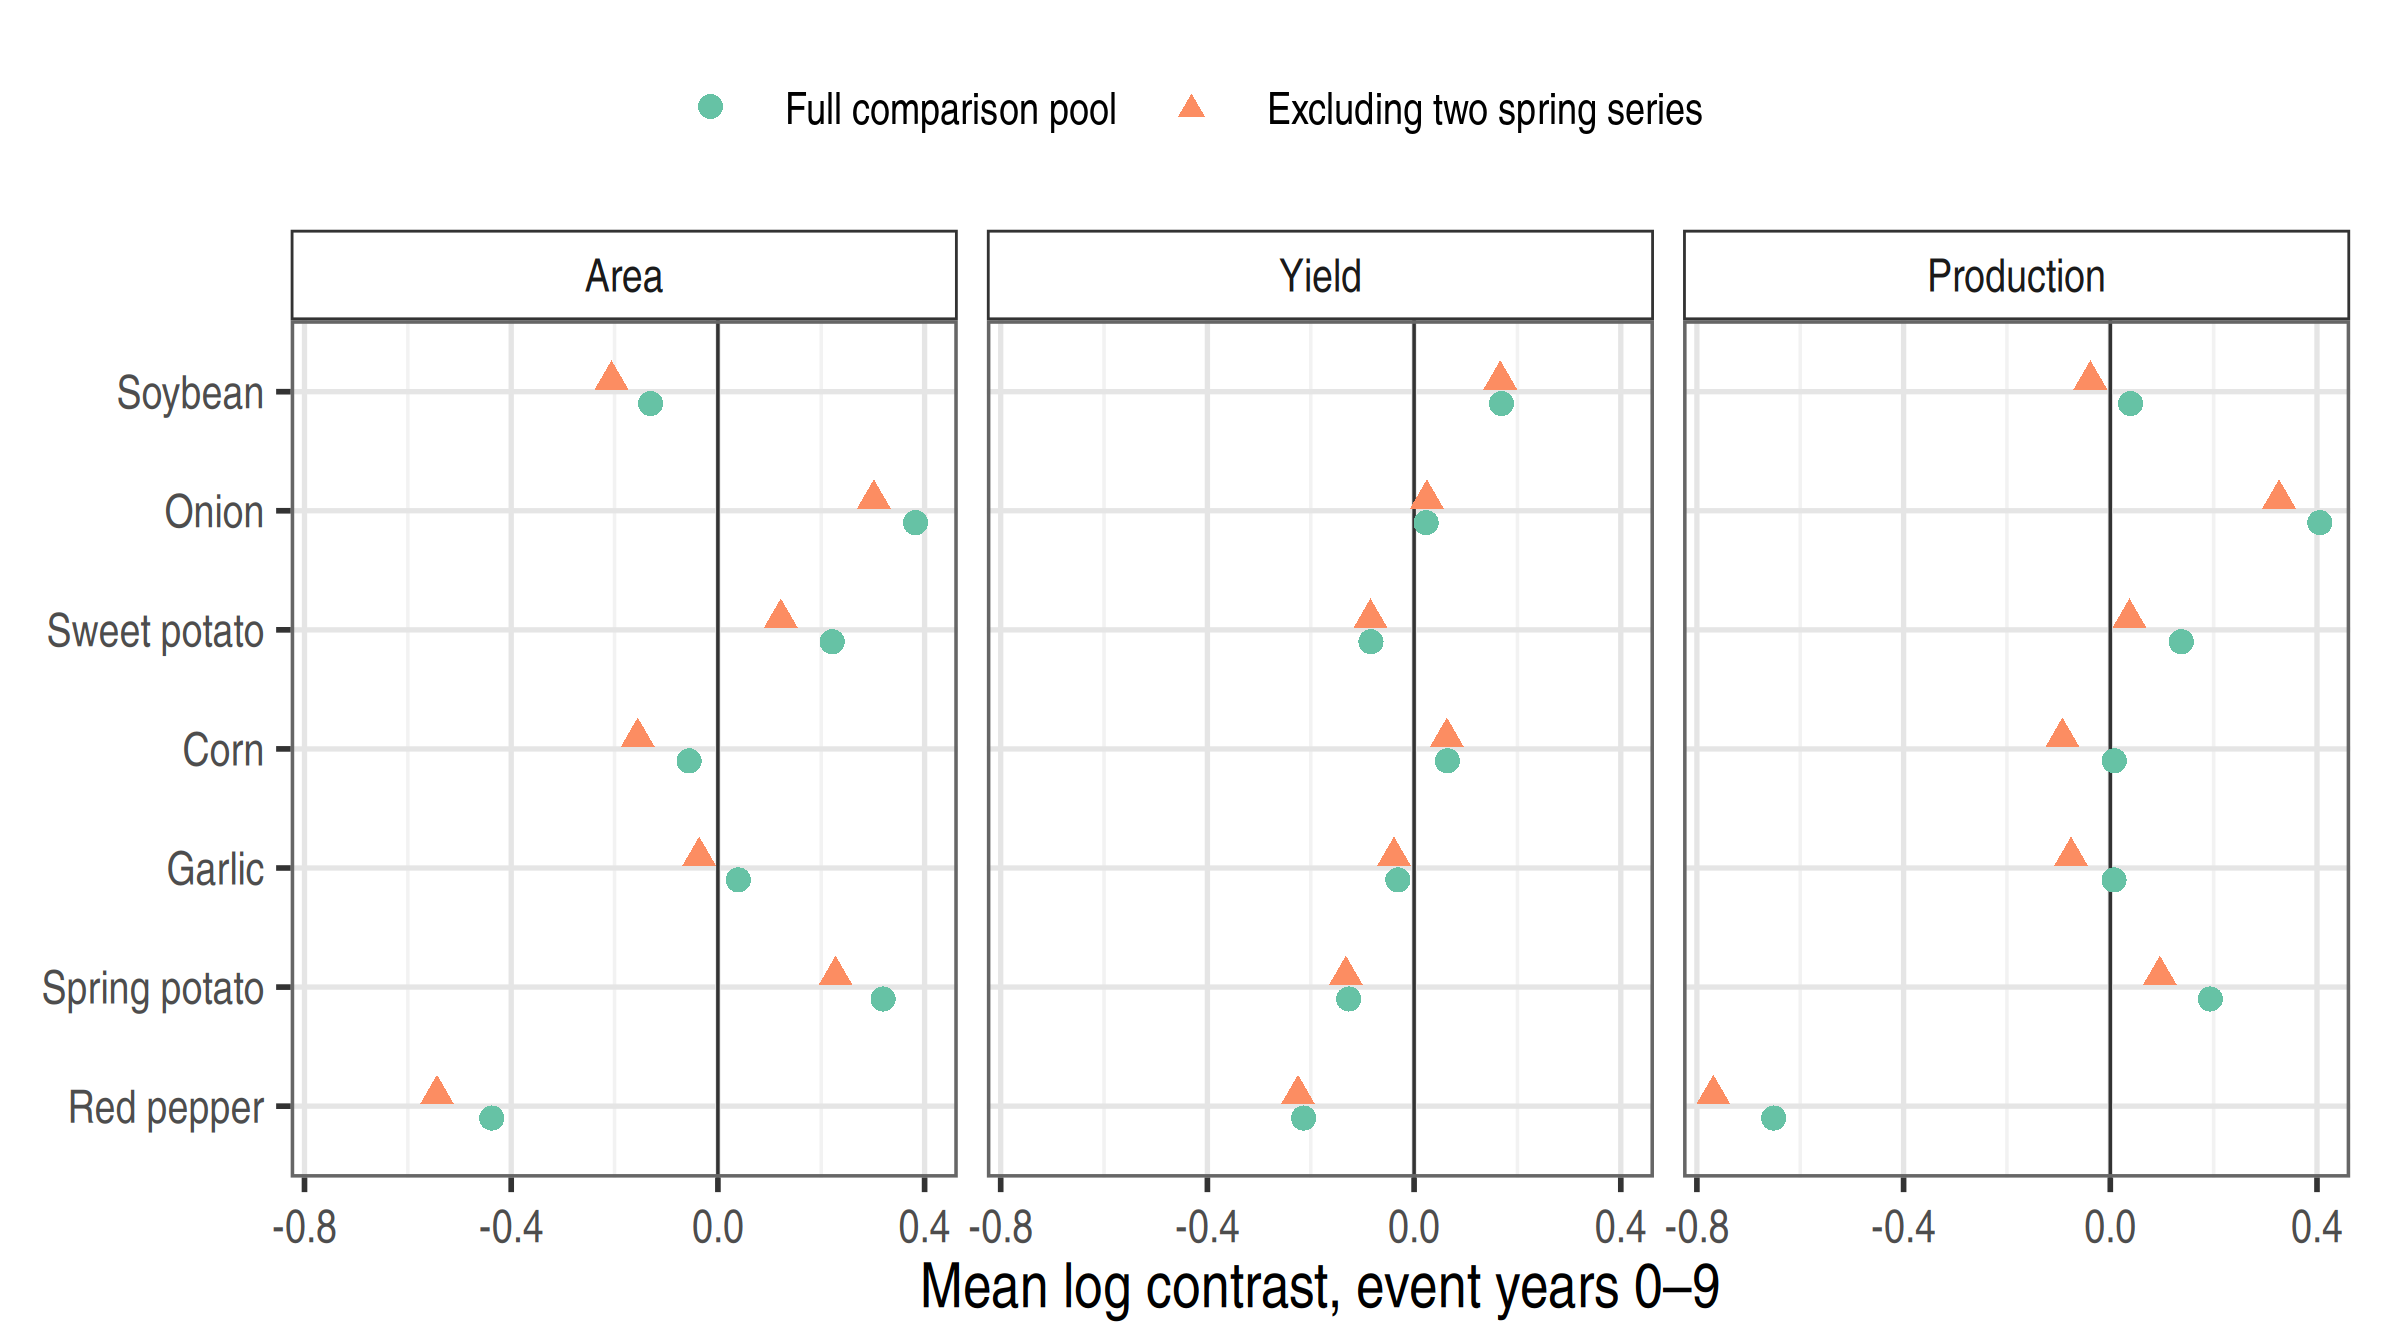
\includegraphics[width=\textwidth]{figures/fig7_crop_contrasts.png}
\caption{Mean Contrasts by Treated Crop}\label{fig:cropcontrasts}
\notes{Each point averages ten crop-specific contrasts. Circles use the full comparison pool, and triangles exclude spring napa cabbage and spring radish. Log points.}
\end{figure}

The small aggregate combines large offsetting contrasts. Production contrasts are 0.406 for onion and 0.193 for spring potato but \textminus 0.651 for red pepper. With equal weights, their respective contributions are approximately 0.058, 0.028, and \textminus 0.093 log points. Omitting one crop at a time moves the aggregate between \textminus 0.044 and 0.132 (Appendix Table~\ref{tab:leaveoneout}). This sensitivity establishes the influence of individual crops, without identifying whether their movements reflect insurance, other shocks, or differences in untreated trends.

\section{Sensitivity to Comparison Choices}\label{sec:sensitivity}

Table~\ref{tab:sensitivity} varies one element of the comparison at a time, keeping the format of Table~\ref{tab:main}.

\begin{table}[htbp]
\centering
\caption{Sensitivity to the Reference Period, Comparison Crops, and Timing}\label{tab:sensitivity}
\begin{tabular*}{\textwidth}{@{\extracolsep{\fill}}lccc}
\toprule
 & (1) & (2) & (3) \\
 & Area & Yield & Production \\
\midrule
\multicolumn{4}{@{}l}{\textit{Panel A. Reference period: mean of last five pre-pilot years}} \\
Contrast & 0.075            & \textminus 0.008          & 0.067 \\
         & (0.150)          & (0.050)           & (0.164) \\
         & [\textminus 0.210, 0.361] & [\textminus 0.105, 0.088] & [\textminus 0.244, 0.378] \\[4pt]
\multicolumn{4}{@{}l}{\textit{Panel B. Reference period: mean of all pre-pilot years}} \\
Contrast & 0.264            & \textminus 0.036          & 0.228 \\
         & (0.184)          & (0.071)           & (0.191) \\
         & [\textminus 0.082, 0.611] & [\textminus 0.170, 0.097] & [\textminus 0.129, 0.585] \\[4pt]
\multicolumn{4}{@{}l}{\textit{Panel C. Comparison crops: field crops only}} \\
Contrast & \textminus 0.054          & \textminus 0.037          & \textminus 0.091 \\
         & (0.187)          & (0.081)           & (0.235) \\
         & [\textminus 0.402, 0.294] & [\textminus 0.190, 0.116] & [\textminus 0.536, 0.354] \\[4pt]
\multicolumn{4}{@{}l}{\textit{Panel D. Comparison crops: excluding uncertain seasonal forms}} \\
Contrast & \textminus 0.082          & \textminus 0.022          & \textminus 0.105 \\
         & (0.154)          & (0.066)           & (0.184) \\
         & [\textminus 0.373, 0.208] & [\textminus 0.146, 0.101] & [\textminus 0.453, 0.243] \\[4pt]
\multicolumn{4}{@{}l}{\textit{Panel E. Timing: product-table years}} \\
Contrast & 0.062            & \textminus 0.025          & 0.036 \\
         & (0.135)          & (0.051)           & (0.153) \\
         & [\textminus 0.192, 0.315] & [\textminus 0.122, 0.072] & [\textminus 0.250, 0.323] \\[4pt]
\multicolumn{4}{@{}l}{\textit{Panel F. Timing: pilot year as start of exposure}} \\
Contrast & 0.034            & \textminus 0.018          & 0.017 \\
         & (0.113)          & (0.045)           & (0.128) \\
         & [\textminus 0.178, 0.247] & [\textminus 0.102, 0.066] & [\textminus 0.224, 0.258] \\
\bottomrule
\end{tabular*}
\notes{Log outcomes; seven treated crops; ten target years; full comparison pool unless stated. Score-based standard errors in parentheses and 95 percent intervals in brackets from 9,999 Webb multiplier draws (Appendix~\ref{app:inference}). * p < 0.10, ** p < 0.05, *** p < 0.01. The main specification is reported in Table~\ref{tab:main}, Panel A. Multi-year references require comparison crops to be observed and not yet exposed in every reference year. Panel D excludes napa cabbage and radish forms, carrot, and green onions, whose survey definitions are uncertain. Panel F dates exposure from the pilot rather than from expansion.}
\end{table}

No specification yields a statistically significant contrast; the smallest p-value, 0.144, belongs to the area contrast with all pre-pilot years as the reference. The reference period and comparison pool nevertheless move the point estimates considerably. Earlier reference periods raise the production contrast to 0.067 and 0.228, as the pre-pilot contrasts in Figure~\ref{fig:eventtime} predict: a longer reference window places the baseline in years when the treated crops were further behind. Restricting the comparison pool lowers the production contrast to \textminus 0.091 or \textminus 0.105, while the timing changes matter less (0.036 and 0.017). The standard errors, between 0.11 and 0.24 for area and production, are large relative to every point estimate, so the specifications differ more in where they center the estimate than in what they can rule out.

Weighting crops by pre-pilot area changes the production contrast from 0.020 to \textminus 0.093, and from \textminus 0.074 to \textminus 0.185 without the two spring series (Table~\ref{tab:areaweights}). Soybean and red pepper receive 61 percent of the weight, whereas onion and spring potato, whose contrasts are positive, receive less. None of the weighted contrasts is statistically significant, and the area-weighted figure is a different summary of the same crop contrasts rather than the percentage change in national production.

\begin{table}[htbp]
\centering
\caption{Contrasts under Pre-Pilot Area Weights}\label{tab:areaweights}
\begin{tabular*}{\textwidth}{@{\extracolsep{\fill}}lccc}
\toprule
 & (1) & (2) & (3) \\
 & Area & Yield & Production \\
\midrule
\multicolumn{4}{@{}l}{\textit{Panel A. Full comparison pool}} \\
Contrast & \textminus 0.091          & \textminus 0.002          & \textminus 0.093 \\
         & (0.151)          & (0.093)           & (0.188) \\
         & [\textminus 0.366, 0.184] & [\textminus 0.165, 0.161] & [\textminus 0.424, 0.238] \\[4pt]
\multicolumn{4}{@{}l}{\textit{Panel B. Excluding two spring series}} \\
Contrast & \textminus 0.179          & \textminus 0.007          & \textminus 0.185 \\
         & (0.141)          & (0.097)           & (0.186) \\
         & [\textminus 0.434, 0.076] & [\textminus 0.177, 0.164] & [\textminus 0.512, 0.141] \\
\bottomrule
\end{tabular*}
\notes{Rows and symbols as in Table~\ref{tab:sensitivity}. Contrasts with equal weights are reported in Table~\ref{tab:main}. Area weights are soybean 36.6, red pepper 24.1, garlic 12.6, sweet potato 7.2, corn 6.8, onion 6.5, and spring potato 6.3 percent; equal weights are 14.3 percent. Comparison crops remain equally weighted within each contrast.}
\end{table}

\section{Municipal Rice Comparison}\label{sec:rice_results}

Table~\ref{tab:riceprepilot} compares the rice cohorts before the pilot. Mean planted area in 2000-2008 was 14,425 hectares among early entrants and 13,666 among later entrants; mean log-area slopes were approximately \textminus 0.011 per year in both groups. Dispersion in area levels was greater among early entrants. Welch tests do not reject equality of the reported means at the 10 percent level.

\begin{table}[htbp]
\centering
\caption{Pre-Pilot Characteristics of Early and Later Rice Municipalities, 2000-2008}\label{tab:riceprepilot}
\begin{tabular*}{\textwidth}{@{\extracolsep{\fill}}lccc}
\toprule
 & (1) & (2) & (3) \\
 & Early entrants & Later entrants & Difference \\
\midrule
Mean planted area, 2000-2008 (ha)        & 14,425   & 13,666   & 759 \\
                                         & (5,871)  & (1,998)  & (1,572) \\
Annual growth of planted area, 2000-2008 & \textminus 0.011 & \textminus 0.011 & \textminus 0.000 \\
                                         & (0.011)  & (0.009)  & (0.004) \\
Change in log planted area, 2000-2008    & \textminus 0.079 & \textminus 0.075 & \textminus 0.003 \\
                                         & (0.077)  & (0.069)  & (0.030) \\
Dispersion around the pre-pilot trend    & 0.017    & 0.012    & 0.005 \\
                                         & (0.012)  & (0.003)  & (0.003) \\
Municipalities                           & 17       & 9        &  \\
\bottomrule
\end{tabular*}
\notes{Columns (1) and (2) report means across municipalities, with standard deviations in parentheses. Column (3) reports the difference in means, with its Welch standard error in parentheses. Annual growth is the least-squares slope of log planted area on year; dispersion around the pre-pilot trend is the standard deviation of the residuals from that trend. * p < 0.10, ** p < 0.05, *** p < 0.01, from Welch t-tests. Data from \citet{statkorea_nd}.}
\end{table}

Table~\ref{tab:rice} reports estimates of equation~\eqref{eq:rice}. The main estimate is \textminus 0.021 log points, with a 95 percent interval of [\textminus 0.064, 0.022], equivalent to approximately \textminus 6.2 to +2.2 percent. In Figure~\ref{fig:riceevent}, pre-pilot coefficients range from approximately \textminus 0.001 to 0.010, with a joint p-value of 0.52. A placebo dated to 2006-2008 within the pre-pilot sample yields 0.001 (p = 0.956).

\begin{table}[htbp]
\centering
\caption{Rice Planted Area in Pilot and Later-Entering Municipalities, 2000-2010}\label{tab:rice}
\begin{tabular*}{\textwidth}{@{\extracolsep{\fill}}lcc}
\toprule
 & (1) & (2) \\
 & Main sample & Excluding weir municipalities \\
\midrule
\textbf{Early entry \texttimes{} Post} & \textminus 0.021          & \textminus 0.002 \\
                                  & (0.022)           & (0.021) \\
                                  & [\textminus 0.064, 0.022] & [\textminus 0.045, 0.039] \\[4pt]
Municipalities (early / later)    & 17 / 9            & 14 / 8 \\
Municipality-years                & 286               & 242 \\
Municipality and year FE          & Yes               & Yes \\
\bottomrule
\end{tabular*}
\notes{The dependent variable is log paddy-rice planted area. Municipality-clustered (CR1) standard errors in parentheses. The 95 percent intervals in brackets and the significance levels are based on the null-imposed wild cluster bootstrap-t with Webb weights, 9,999 draws, and municipality clusters. * p < 0.10, ** p < 0.05, *** p < 0.01. Column (2) excludes Gumi, Sangju, Naju, and Uiseong, municipalities adjoining weirs built under the Four Major Rivers Restoration Project \citep{kwater}.}
\end{table}

Excluding Gumi, Sangju, Naju, and Uiseong, municipalities adjoining weirs built under the Four Major Rivers Restoration Project, moves the estimate to \textminus 0.002 (p = 0.940). The estimate is therefore sensitive to the municipalities represented. This exclusion changes the sample rather than separately estimating the effect of river works. As a sensitivity check, province-clustered CR1 inference yields p = 0.387 using a t distribution with seven degrees of freedom. With only eight province clusters, this result remains subject to small-cluster uncertainty.

\begin{figure}[htbp]
\centering
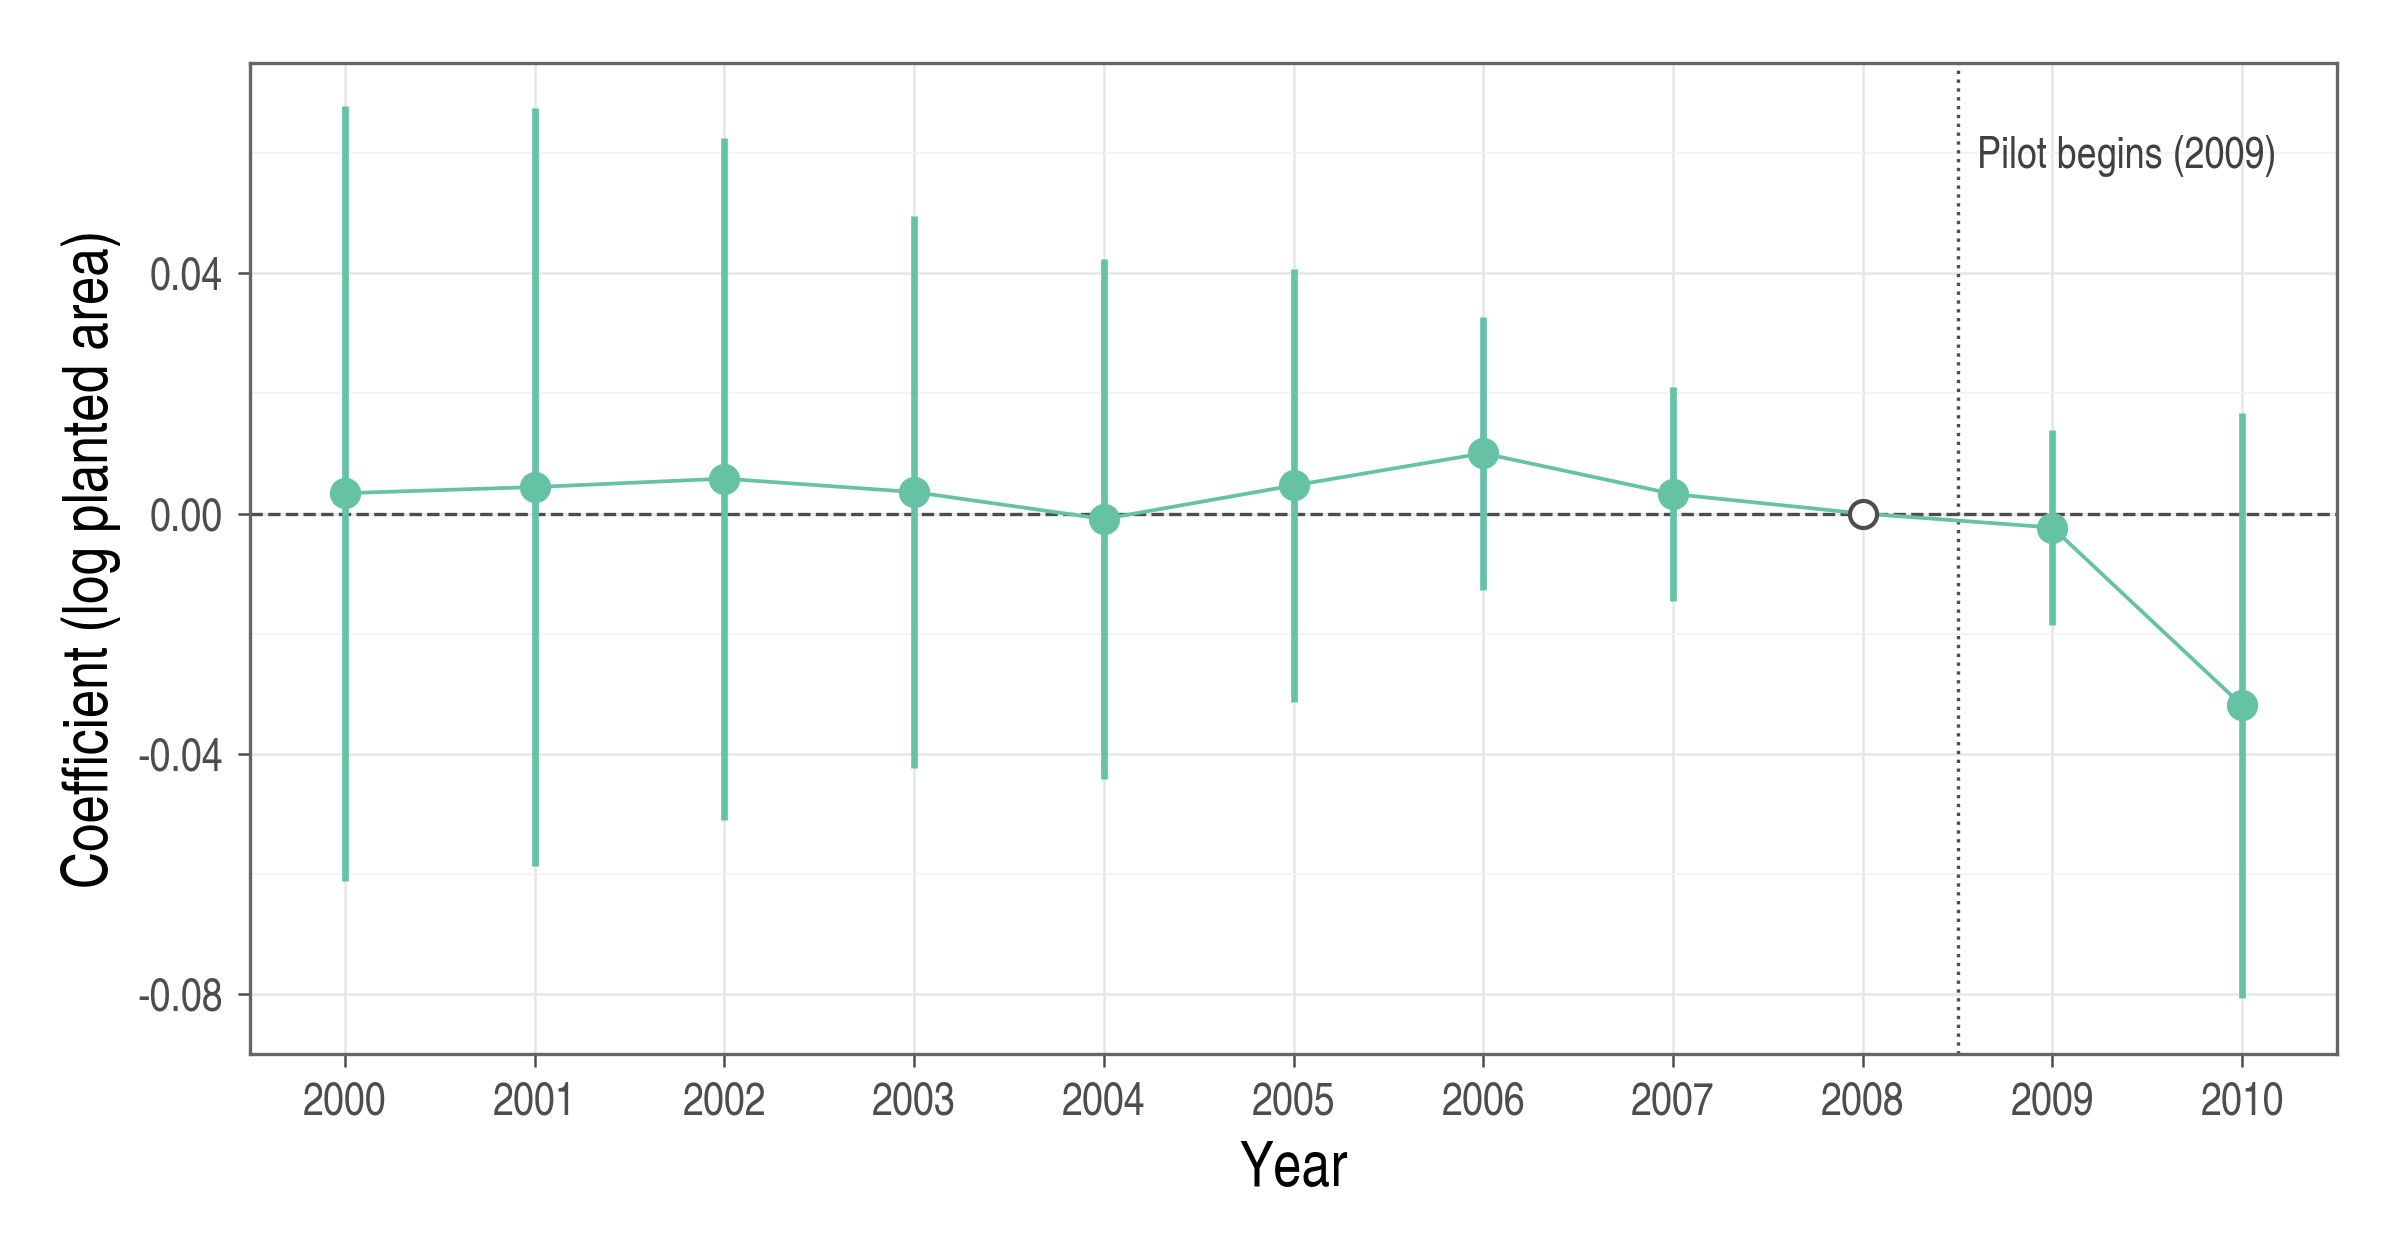
\includegraphics[width=\textwidth]{figures/fig8_rice_event_study.png}
\caption{Event-Study Coefficients for Rice Planted Area, 2000-2010}\label{fig:riceevent}
\notes{Coefficients from a regression of log paddy-rice planted area on municipality and year fixed effects and interactions of early-entry status with year indicators; 2008 is the reference year (open circle). Bars are 95 percent confidence intervals based on municipality-clustered (CR1) standard errors with t(25) critical values; they differ from the wild bootstrap intervals in Table~\ref{tab:rice}. The sample comprises 17 early and nine later-entering municipalities over 2000-2010.}
\end{figure}

\section{Comparability of Treated and Comparison Crops}\label{sec:comparability}

Table~\ref{tab:pregrowth} compares pre-pilot slopes for the seven treated and 22 contributing comparison crops. Mean log-area slopes were \textminus 0.015 and \textminus 0.046 per year, respectively; production slopes were \textminus 0.005 and \textminus 0.031. Yield slopes were closer, at 0.010 and 0.015. Standardized differences are 0.87 for area, 0.71 for production, and \textminus 0.31 for yield. The larger area and production gaps reinforce the pre-pilot divergence in Figure~\ref{fig:eventtime}.

\begin{table}[htbp]
\centering
\caption{Pre-Pilot Growth of Treated and Comparison Crops, 1998-2007}\label{tab:pregrowth}
\begin{tabular*}{\textwidth}{@{\extracolsep{\fill}}lcccc}
\toprule
 & (1) & (2) & (3) & (4) \\
 & \shortstack{Treated\\crops} & \shortstack{Comparison\\crops} & Difference & \shortstack{Std.\\difference} \\
\midrule
Annual growth of cultivated area & \textminus 0.015 & \textminus 0.046 & 0.031    & 0.867 \\
                                 & (0.022)  & (0.045)  &          &  \\
Annual growth of yield           & 0.010    & 0.015    & \textminus 0.005 & \textminus 0.313 \\
                                 & (0.019)  & (0.014)  &          &  \\
Annual growth of production      & \textminus 0.005 & \textminus 0.031 & 0.026    & 0.706 \\
                                 & (0.022)  & (0.046)  &          &  \\
Crop series                      & 7        & 22       &          &  \\
\bottomrule
\end{tabular*}
\notes{Unweighted means of crop-specific least-squares slopes of log outcomes on year over 1998-2007; standard deviations across crops in parentheses. Difference is the treated mean minus the comparison mean. Standardized difference divides that gap by the square root of the average of the two group variances; it is descriptive, not a test statistic. Large and small green onions have eight annual observations; other crops have ten.}
\end{table}

Changing the reference period or comparison pool changes the growth histories against which treated crops are evaluated. The pre-pilot differences help explain the comparisons underlying the national sensitivity results. The municipal design holds crop identity fixed and instead compares regional growth histories.
